\tikzstyle{vertex}=[draw,black,fill=blue,circle,minimum size=24pt,inner sep=0pt]
\tikzstyle{edge}=[very thick]
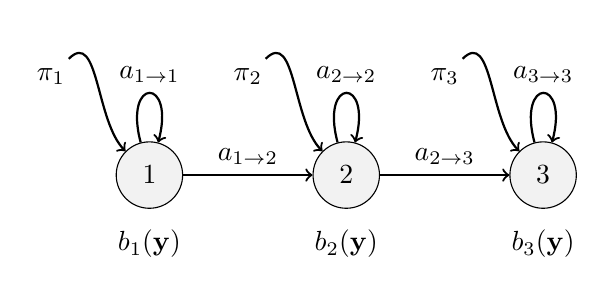
\begin{tikzpicture}[scale=2.5]
    \node (a)[vertex,fill=gray!10,align=left] at (0,0) {$1$};
    \node (b)[vertex,fill=gray!10,align=left] at (1,0)  {$2$};
    \node (c)[vertex,fill=gray!10,align=left] at (2,0)  {$3$};
    \node (pi1) at (-0.5,0.5) {$\pi_1$};
    \node (pi2) at (0.5,0.5) {$\pi_2$};
    \node (pi3) at (1.5,0.5) {$\pi_3$};
    \node (b1) at (0,-0.35) {$b_1(\mathbf{y})$};
    \node (b2) at (1,-0.35) {$b_2(\mathbf{y})$};
    \node (b3) at (2,-0.35) {$b_3(\mathbf{y})$};
    \path[thick,->] (a)    edge node [anchor=center,above,sloped] {$a_{1 \rightarrow 2}$} (b);
    \path[thick,->] (b)    edge node [anchor=center,above,sloped] {$a_{2 \rightarrow 3}$} (c);
    \path[thick,->] (a)    edge[loop above, looseness=10] node [anchor=center,above,sloped] {$a_{1 \rightarrow 1}$} (a);
    \path[thick,->] (b)    edge[loop above, looseness=10] node [anchor=center,above,sloped] {$a_{2 \rightarrow 2}$} (b);
    \path[thick,->] (c)    edge[loop above, looseness=10] node [anchor=center,above,sloped] {$a_{3 \rightarrow 3}$} (c);
    \path[thick,->] (pi1)  edge[looseness=1] node [anchor=center,above,sloped] {} (a);
    \path[thick,->] (pi2)  edge[looseness=1] node [anchor=center,above,sloped] {} (b);
    \path[thick,->] (pi3)  edge[looseness=1] node [sloped] {} (c);
\end{tikzpicture}
